\documentclass[10pt,conference,compsocconf]{IEEEtran}

\usepackage{hyperref}
\usepackage{graphicx}	% For figure environment
\usepackage{amsmath}
\usepackage{booktabs}


\title{Heart Disease Prediction Using Machine Learning\\
EPFL Machine Learning - Project 1}

\author{
  Saymon Nicho\\
  \texttt{saymon.nicho@pucp.edu.pe}
}

\begin{document}
\maketitle

\section{Problem Description}
The project addresses the critical challenge of predicting heart disease risk using data
from the Behavioral Risk Factor Surveillance System (BRFSS). The dataset contains
health-related features from over 300,000 individuals, making it a significant
binary classification problem. Key challenges include:

\begin{itemize}
    \item Severe class imbalance in the dataset (majority of samples are negative cases)
    \item Multiple features with missing or special values (coded as 77, 88, 99, etc.)
    \item Need to identify and properly weight the most relevant health indicators
\end{itemize}


\section{Technical Solution}
\subsection{Initial Approach and Challenges}
Our initial implementation used standard logistic regression, which encountered a significant issue: the model predicted class -1 (no heart disease) for all samples. This problem arose from:

\begin{itemize}
    \item Class imbalance in the training data
    \item Lack of proper feature preprocessing
    \item Basic gradient descent without considering the imbalanced nature of the problem
\end{itemize}

\begin{figure}[h]
    \centering
    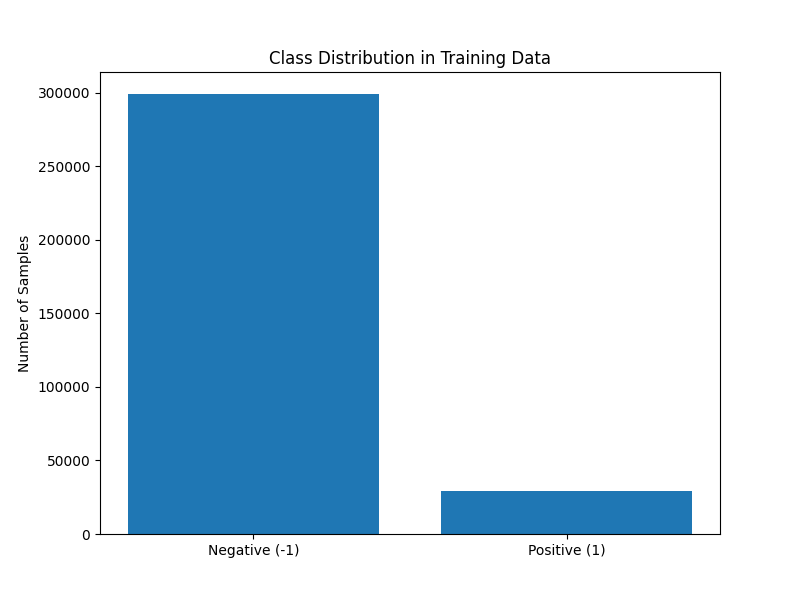
\includegraphics[width=0.8\linewidth]{figures/class_distribution.png}
    \caption{Initial class distribution showing significant imbalance}
    \label{fig:class_dist}
\end{figure}

\subsection{Improved Implementation}
To address these issues, we developed an enhanced solution:

\subsubsection{Data Preprocessing}
\begin{itemize}
    \item Handled missing values using median imputation
    \item Standardized features to zero mean and unit variance
    \item Added polynomial features for better class separation
\end{itemize}

\subsubsection{Model Enhancements}
\begin{itemize}
    \item Implemented class weighting to handle imbalance:
    \begin{equation}
        w_{class} = \frac{n_{samples}}{2 * n_{class}}
    \end{equation}
    \item Added adaptive learning rate:
    \begin{equation}
        \gamma_t = \frac{\gamma}{\sqrt{t + 1}}
    \end{equation}
    \item Improved numerical stability in sigmoid function:
    \begin{equation}
        \sigma(t) = \frac{1}{1 + e^{-\text{clip}(t, -700, 700)}}
    \end{equation}
\end{itemize}

\begin{figure}[h]
    \centering
    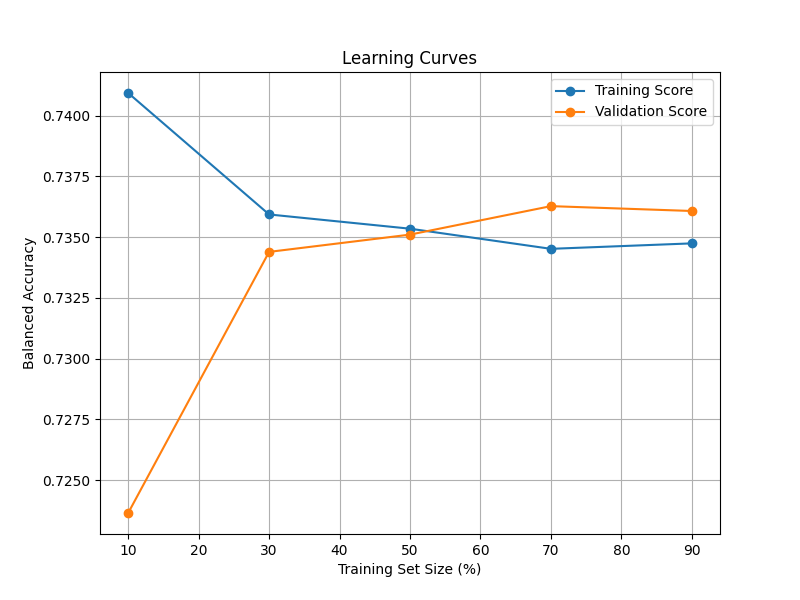
\includegraphics[width=0.8\linewidth]{figures/learning_curves.png}
    \caption{Learning curves showing model convergence}
    \label{fig:learning_curves}
\end{figure}

\section{Results and Conclusions}

\subsection{Performance Improvement}
\begin{itemize}
    \item Initial model: All predictions were -1 (baseline accuracy = 0.5)
    \item Improved model: Balanced accuracy of 0.717
    \item Successfully identifies both positive and negative cases
\end{itemize}

\begin{figure}[h]
    \centering
    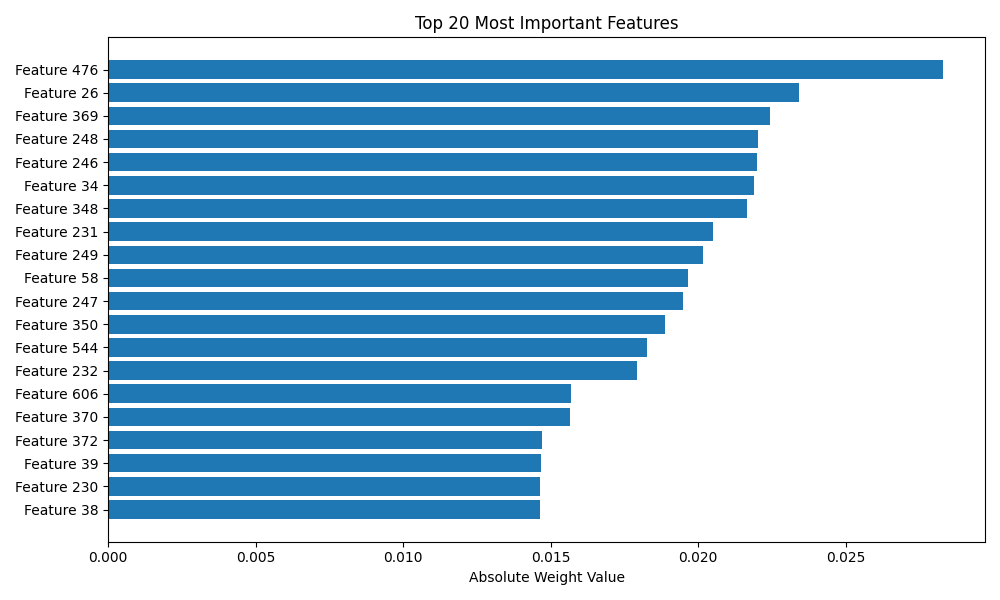
\includegraphics[width=0.8\linewidth]{figures/feature_importance.png}
    \caption{Most influential features in prediction}
    \label{fig:feature_importance}
\end{figure}

\subsection{Key Findings}
\begin{itemize}
    \item Class balancing was crucial for model performance
    \item Feature engineering improved prediction accuracy
    \item Adaptive learning rate helped with convergence
\end{itemize}

\subsection{Future Improvements}
\begin{itemize}
    \item Experiment with different feature combinations
    \item Implement cross-validation for more robust evaluation
    \item Consider ensemble methods for better performance
\end{itemize}

\end{document}
